% !TeX spellcheck = ru_RU
% !TEX root = vkr.tex

\section{Обзор}
\label{sec:relatedworks}

В этом разделе рассматривается контекст, необходимый для формулировки
требований к байткодной виртуальной машине Lama. Сначала кратко описываются
свойства самого языка, которые влияют на исполнение программ: единое
представление значений, работа с составными объектами, функции, замыкания и
модульность. Затем разбирается существующая инфраструктура языка Lama. В завершение обсуждаются ограничения
текущего интерпретатора и общие архитектурные решения, применимые к стековым
виртуальным машинам.

\subsection{Обзор языка Lama}

Lama --- учебный язык программирования, разработанный для изучения устройства языков
программирования, компиляторов и сред исполнения. Описание языка и его открытая реализация доступны
в репозитории проекта и спецификации языка~\cite{LamaReadme,LamaSpec}. 

В языке присутствуют различного рода конструкции: изменяемые переменные, операторы присваивания,
условные операторы, циклы и последовательное исполнение выражений, функции как значения. Кроме того,
в языке есть составные структуры данных: массивы, строки, S-выражения и сопоставление с образцом. 

Исходный байткод Lama задаёт стековую модель вычислений: инструкции берут аргументы со стека и
помещают результат обратно на стек. На уровне выполнения программа Lama оперирует единым
представлением значений. Часть значений может храниться непосредственно на стеке, а составные
объекты размещаются в куче и обслуживаются средой выполнения.

Отдельно важна модульная система. Практическая программа на Lama может состоять из нескольких
модулей, импортирующих функции и значения друг друга. Это влияет на байткодное исполнение: запуск
программы в общем случае связан не только с одним файлом, но и с загрузкой нескольких модулей,
регистрацией публичных символов и разрешением внешних ссылок. Без учета этой особенности байткодная
реализация остается ограниченной и не отражает полный сценарий использования языка.

\subsection{Существующая инфраструктура языка Lama}

Существующая инфраструктура языка Lama организована вокруг компилятора, среды выполнения и
стандартной библиотеки \cite{LamaReadme}. Точкой входа служит \verb=Driver.ml=: он разбирает
программу через \verb=Language.run_parser= и в зависимости от параметров запуска выбирает один из
путей исполнения или компиляции.

\begin{figure}[H]
    \centering
    \resizebox{\textwidth}{!}{\begin{tikzpicture}[
    x=1cm,
    y=1cm,
    stage/.style={
        draw,
        rounded corners=2pt,
        semithick,
        align=center,
        minimum height=11mm,
        text width=32mm,
        fill=gray!8
    },
    transform/.style={
        draw,
        rounded corners=2pt,
        semithick,
        align=center,
        minimum height=11mm,
        text width=32mm,
        fill=gray!8
    },
    snippetstage/.style={
        draw,
        line width=0.35pt,
        draw=black!30,
        minimum width=37mm,
        minimum height=24mm,
        fill=white
    },
    smstage/.style={
        draw,
        line width=0.35pt,
        draw=black!30,
        minimum width=37mm,
        minimum height=24mm,
        fill=white
    },
    component/.style={
        draw,
        rounded corners=2pt,
        line width=0.35pt,
        draw=black!35,
        align=center,
        minimum height=10mm,
        text width=34mm,
        fill=gray!8
    },
    support/.style={
        draw,
        rounded corners=2pt,
        semithick,
        align=center,
        minimum height=11mm,
        text width=37mm,
        fill=blue!10
    },
    test/.style={
        draw,
        rounded corners=2pt,
        semithick,
        align=center,
        minimum height=11mm,
        text width=37mm,
        fill=green!12
    },
    result/.style={
        draw,
        rounded corners=2pt,
        line width=0.35pt,
        draw=black!35,
        align=center,
        minimum height=10mm,
        text width=34mm,
        fill=orange!14
    },
    note/.style={
        align=center,
        font=\small,
        text width=38mm
    },
    resultlabel/.style={
        align=center,
        font=\small
    },
    flow/.style={->, semithick},
    attach/.style={->, dashed, semithick}
]

\node[snippetstage] (source) at (0,0) {};
\node[transform] (driver) at (4.4,0) {драйвер\\компилятора};
\node[transform, text width=38mm] (language) at (8.6,0) {лексический и\\синтаксический\\анализ};
\node[smstage] (stack) at (13.1,0) {};

\node[anchor=north west, inner sep=0pt] at ($(source.north west)+(0.8mm,-0.8mm)$) {
    \begin{tikzpicture}[x=1mm,y=-1mm]
        \clip (0,0) rectangle (36.4,21.9);
        \node[
            anchor=north west,
            align=left,
            font=\ttfamily\fontsize{4.6}{5.1}\selectfont
        ] at (0.05,0.05)
            {var x, y, z;\\
             \\
             fun zip (x) \{\\
             \ \ case x of Pair (x, y) ->\\
             \ \ \ \ case x of\\
             \ \ \ \ \ \ Nil          ->  Nil\\
             \ \ \ \ | Cons (x, xs) -> case y of\\
             \ \ \ \ \ \ \ \ \ \ \ \ \ \ \ Nil ->  Nil\\
             \ \ \ \ \ \ \ \ \ \ \ \ \ \ | Cons (y, ys) ->\\
             \ \ \ \ \ \ \ \ \ \ \ \ \ \ \ \ Cons (Pair (x, y),\\
             \ \ \ \ \ \ \ \ \ \ \ \ \ \ \ \ \ \ zip (Pair (xs, ys)))\\
             \ \ \ \ \ \ \ \ \ \ \ \ \ \ esac\\
             \ \ \ \ esac};
        \node[anchor=south east, font=\ttfamily\tiny, text=gray!65]
            at (36.8,21.5) {$\ddots$};
    \end{tikzpicture}
};
\node[font=\small, align=center, below=1mm of source] {исходная\\программа};

\node[anchor=north west, inner sep=0pt] at ($(stack.north west)+(0.8mm,-0.8mm)$) {
    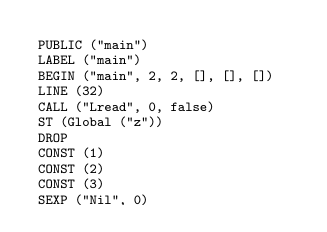
\begin{tikzpicture}[x=1mm,y=-1mm]
        \clip (0,0) rectangle (34.4,22.4);
        \node[
            anchor=north west,
            align=left,
            font=\ttfamily\fontsize{5.0}{5.6}\selectfont
        ] at (0.1,0.25)
            {PUBLIC ("main")\\
             LABEL ("main")\\
             BEGIN ("main", 2, 2, [], [], [])\\
             LINE (32)\\
             CALL ("Lread", 0, false)\\
             ST (Global ("z"))\\
             DROP\\
             CONST (1)\\
             CONST (2)\\
             CONST (3)\\
             SEXP ("Nil", 0)\\
             SEXP ("Cons", 2)};
    \end{tikzpicture}
};

\node[component] (native-backend) at (13.1,2.7) {нативная\\генерация кода};
\node[resultlabel] (native-code) at (17.2,2.7) {нативный код};
\node[support, fill=gray!12, text width=32mm] (execenv) at (15.2,4.4) {среда выполнения};
\node[support, fill=gray!12, text width=32mm] (stdlib) at (19.2,4.4) {стандартная\\библиотека};

\node[resultlabel] (bytecode) at (17.2,0) {байткод};
\node[resultlabel] (stackinterp) at (13.1,-2.8) {интерпретация\\стекового представления};
\node[resultlabel] (sourceinterp) at (8.6,-2.8) {интерпретация\\исходного языка};

% \node[test, text width=34mm] (tests) at (4.4,2.7) {регрессионные\\тесты};

\draw[flow] (source) -- (driver);
\draw[flow] (driver) -- (language);
\draw[flow] (language) -- (stack);

\draw[flow] (stack) -- (native-backend);
\draw[flow] (native-backend) -- (native-code);
\draw[flow] (stack) -- (bytecode);
\draw[flow] (stack) -- (stackinterp);
\draw[flow] (language) -- (sourceinterp);

\draw[attach]   (native-code) -- (execenv);
\draw[attach]  (native-code) -- (stdlib);
% \draw[attach] (tests) -- (driver);

\end{tikzpicture}
}
    \caption{Архитектура существующей инфраструктуры Lama на уровне основных представлений и путей исполнения.}
    \label{fig:lama-current-infrastructure}
\end{figure}

По умолчанию и в режиме
\verb=-c= драйвер выбирает нативный бэкенд для архитектуры X86\_64. Этот бэкенд также
использует стековое представление: сначала программа преобразуется через
\verb=SM.compile=, а затем полученный стековый код транслируется в нативный
код. В режиме \verb=-b= то же стековое представление записывается как байткод
через \verb=SM.ByteCode.compile=. В режиме \verb=-s= оно выполняется
интерпретатором \verb=SM.run=. Режим \verb=-i= обходит стековую машину и
запускает исходный уровень через \verb=Language.eval=. Таким образом,
\verb=Language.ml= отвечает не только за лексический и синтаксический анализ
программы, но и за отдельный путь интерпретации исходного языка, тогда как
\verb=SM.ml= является общей точкой для нативной генерации, байткодной
генерации и стекового исполнения.

Нативная ветка связана с существующей средой выполнения. В репозитории есть
отдельные исходные коды для 64-битной сборки, а реализация сборщика
мусора находится в \verb=gc.c=. Каталог \verb=stdlib/= содержит модули стандартной
библиотеки языка Lama; в
существующей инфраструктуре они относятся прежде всего к нативной сборке
программ, где поддерживаются импорты и связывание с объектными файлами
стандартной библиотеки.

Байткод в этой инфраструктуре является сериализованной формой стекового
представления. В нем уже нет многих поверхностных конструкций языка, но
сохраняются операции загрузки констант, работы со стеком, обращения к локальным
и глобальным значениям, вызова функций, создания замыканий, условных и
безусловных переходов, а также сопоставления с образцом.

\subsection{Ограничения существующего интерпретатора}

Существующий путь интерпретации стекового представления реализован в
\verb=SM.ml= на OCaml~\cite{LamaInterpreter,OCamlManual}. Он полезен как часть
компиляторной инфраструктуры, однако не решает все задачи самостоятельного
байткодного исполнения.

Первое ограничение связано с полнотой сценария запуска. В существующей
инфраструктуре программы с импортами и стандартной библиотекой поддерживаются
только нативной сборкой. Поэтому байткодное исполнение в общем случае требует
отдельной поддержки загрузки модулей, регистрации публичных символов и
разрешения межмодульных ссылок.

Второе ограничение связано с интеграцией со средой выполнения. Среда
выполнения Lama задает представление значений, соглашения о выделении памяти,
интерфейс сборщика мусора и набор встроенных функций. Интерпретатор на OCaml находится в
другой среде исполнения, поэтому его прямое использование как байткодной
виртуальной машины не дает той же модели взаимодействия со средой выполнения,
что и нативный путь.

Наконец, существующий интерпретатор является частью компилятора, а не
самостоятельной платформой для экспериментов с байткодным исполнением. Это
ограничивает исследование таких аспектов, как внутреннее представление
инструкций, диспетчеризация, организация стека и предварительная проверка
байткода. 

\subsection{Подходы к организации виртуальных машин}

В этом подразделе рассматриваются архитектурные решения, определяющие представление инструкций, модель вычислений, состояние исполнения и связь виртуальной машины со средой исполнения.

\subsubsection{Представление исполняемых инструкций}
При проектировании байткодного исполнителя важен способ представления
исполняемых инструкций~\cite{Shi}. Самый прямой вариант --- выполнять байтовый
поток непосредственно: цикл интерпретатора считывает очередной код операции,
выбирает ветку обработки и декодирует операнды по мере исполнения. Такой
подход прост и хорошо подходит для минимальной реализации, но часть работы
повторяется при каждом выполнении инструкции. Кроме того, цели переходов,
ссылки на функции и обращения к внешним символам приходится разрешать внутри
основного цикла или рядом с ним.

Альтернативный подход состоит в предварительной конвертации байткода во внутреннее представление
инструкций~\cite{dram2024threaded, ThreadedCode}. На этапе загрузки
байткод декодируется один раз, операнды приводятся к удобной для исполнения
форме, цели переходов заменяются указателями или индексами внутренних
инструкций, а внешние ссылки разрешаются через таблицу символов. После этого
основной цикл работает уже с подготовленным массивом инструкций. Такой подход
увеличивает объем предварительной обработки, но упрощает исполнение и
позволяет раньше обнаруживать ошибки в байткоде.

\subsubsection{Организация состояния исполнения}
Другой важный выбор связан с моделью вычислений. Виртуальные машины часто
разделяют на стековые и регистровые~\cite{Shi, Simek}. В стековой машине
операнды неявно берутся с вершины стека и результат также помещается на стек.
Это делает инструкции компактными и хорошо соответствует байткоду языка Lama, где
многие операции уже имеют стековую форму. Регистровая машина хранит значения в
явно адресуемых виртуальных регистрах; такой формат может уменьшать число
операций со стеком, но требует другого представления кода и более сложного
выбора операндов.

Модель вычислений связана с устройством состояния исполнения. Для языка с
функциями, локальными переменными, аргументами, замыканиями и сборщиком мусора
одного абстрактного стека операндов недостаточно. Виртуальная машина должна
представлять кадры вызова, адрес возврата, границы локальных переменных,
глобальные области модулей и значения, видимые сборщику мусора как корни.
Возможны разные варианты: отдельный стек вызовов, единый стек значений с
базовым указателем кадра или динамически выделяемые кадры. Для языка Lama особенно
важна совместимость со средой исполнения, поэтому состояние виртуальной машины
должно быть организовано так, чтобы сборщик мусора мог корректно сканировать
активные значения.

\subsubsection{Взаимодействие со средой исполнения}
Отдельную часть архитектуры образует взаимодействие с внешними функциями.
Значительная часть встроенной функциональности уже реализована в среде
исполнения языка Lama, и виртуальная машина может переиспользовать эту логику.
Возможны прямые вызовы заранее известных функций, таблица встроенных операций
или более общий механизм разрешения внешних символов. Библиотека
\texttt{libffi} показывает распространенный подход к такой задаче: она
предоставляет переносимый интерфейс для вызова функций с соглашениями о
вызовах, которые зависят от платформы и могут быть описаны во время
выполнения~\cite{Libffi}. Для обратных вызовов в подобных интерфейсах также
используются замыкания и трамплины, связывающие адрес, ожидаемый кодом на C, с
обработчиком в среде исполнения. Для модульного байткода особенно важно, чтобы
ссылки на внешние функции разрешались явно и ошибки отсутствующих символов
обнаруживались до или во время подготовки программы к исполнению, а не
приводили к неопределенному поведению.


\subsection{Выводы}

Проведенный обзор показывает, что для Lama недостаточно реализовать только
набор обработчиков байткодных инструкций. На устройство байткодного исполнения
влияют модульная система, существующая среда исполнения, представление значений языка и
необходимость устойчивой обработки бинарного входа.

Ограничения существующего интерпретатора делают целесообразной
реализацию новой виртуальной машины на C. Такая реализация может быть ближе к
среде выполнения Lama, явно управлять стеком и кадрами вызова, использовать
существующие встроенные функции и предоставлять основу для дальнейшего
тестирования и оптимизации байткодного исполнения.
